% Основная часть отчёта по лабораторной работе №3

\chapter{Постановка задачи}
Цель работы: исследовать цифровую САУ температуры, синтезировать и настроить дискретный регулятор согласно порядку выполнения из методички (стр. 49–56). Вариант: \textbf{8} (табл.~7: $T_1=0{,}9$, $T_2=1{,}05$).

\section{Модель объекта и выбор периода дискретизации}
Непрерывная часть объекта представляется последовательно соединёнными звеньями вида $\frac{1}{T_1 s + 1}$ и $\frac{1}{T_2 s + 1}$.
Период дискретизации выбираем по заданию: сначала $T = T_1/2$, затем $T=T_1/4$. В качестве датчика используем ZOH.

\section{Синтез дискретного регулятора}
Для структуры согласно рис.~17–18 методички выполняется расчёт параметров регулятора и подбор коэффициента передачи $q_0$, обеспечивающего слабоколебательный процесс. Моделирование и поиск $q_0$ выполняются в Python (см. листинги), графики приведены ниже.

Методика подбора $q_0$ (в соответствии с п.~2–3 порядка работ):
\begin{enumerate}
    \item фиксируем период дискретизации $T$ (сначала $T=T_1/2$, затем $T=T_1/4$) и дискретизуем объект через ZOH;
    \item проводим серию моделирований по сетке $q_0\in[q_{\min}, q_{\max}]$;
    \item выбираем $q_0$, обеспечивающий перерегулирование в пределах 5–15\% и минимальное время установления (если таких нет, берём минимум по интегральному критерию ISE при устойчивости).
\end{enumerate}
По результатам подбора: при $T=T_1/2$ получено $q_0\approx4.00$, при $T=T_1/4$ — $q_0\approx4.92$.

\section{Эксперименты}
Для каждого из периодов дискретизации проведены три эксперимента:
\begin{enumerate}
    \item реакция на ступенчатое задающее воздействие;
    \item реакция на ступенчатое возмущающее воздействие;
    \item реакция на возмущение, изменяющееся по случайному закону.
\end{enumerate}

\begin{figure}[H]
    \centering
    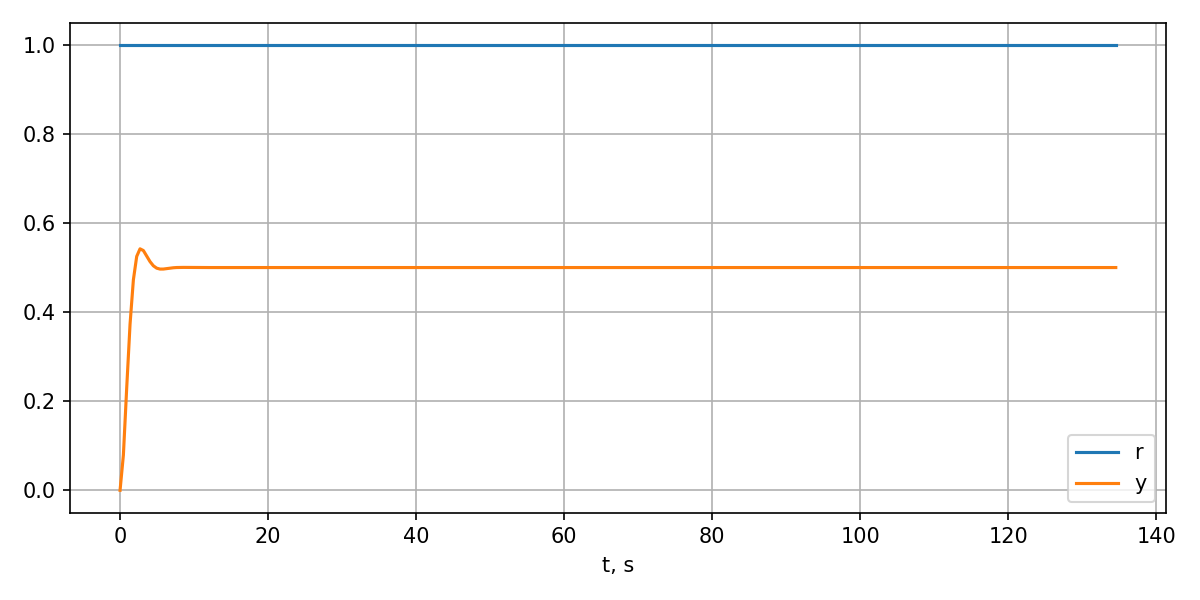
\includegraphics{task1/step_set_T12.png}
    \caption{Ступенчатое задание, $T=T_1/2$}
\end{figure}

\begin{figure}[H]
    \centering
    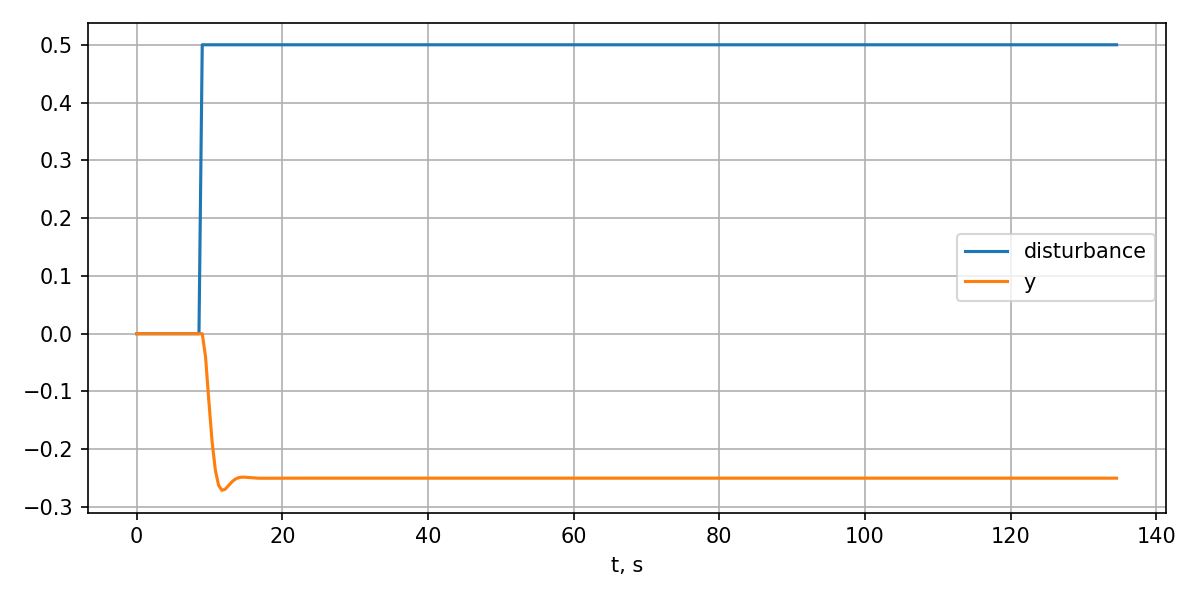
\includegraphics{task1/step_dist_T12.png}
    \caption{Ступенчатое возмущение, $T=T_1/2$}
\end{figure}

\begin{figure}[H]
    \centering
    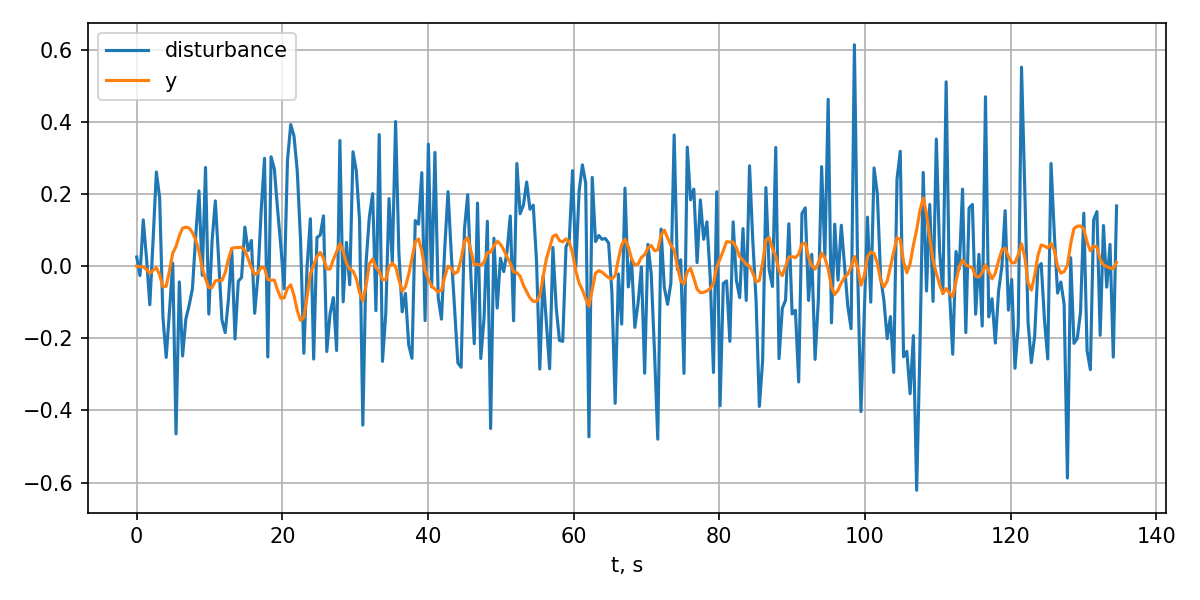
\includegraphics{task1/noise_T12.png}
    \caption{Случайное возмущение, $T=T_1/2$}
\end{figure}

Для $T=T_1/4$ получены аналогичные результаты (см. ниже):

\begin{figure}[H]
    \centering
    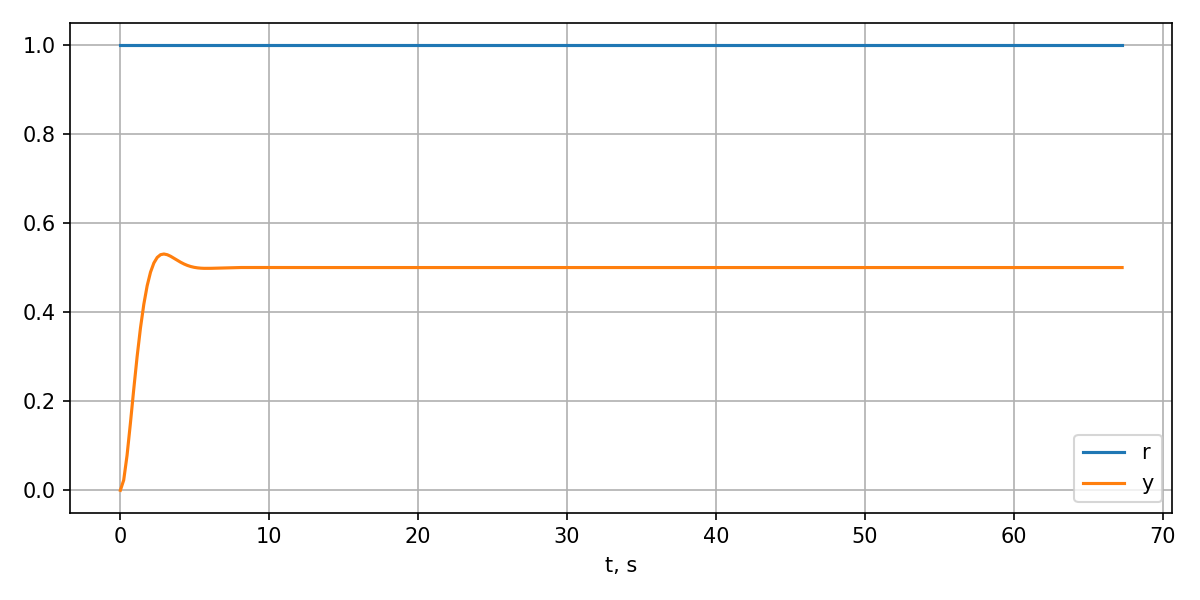
\includegraphics{task1/step_set_T14.png}
    \caption{Ступенчатое задание, $T=T_1/4$}
\end{figure}

\begin{figure}[H]
    \centering
    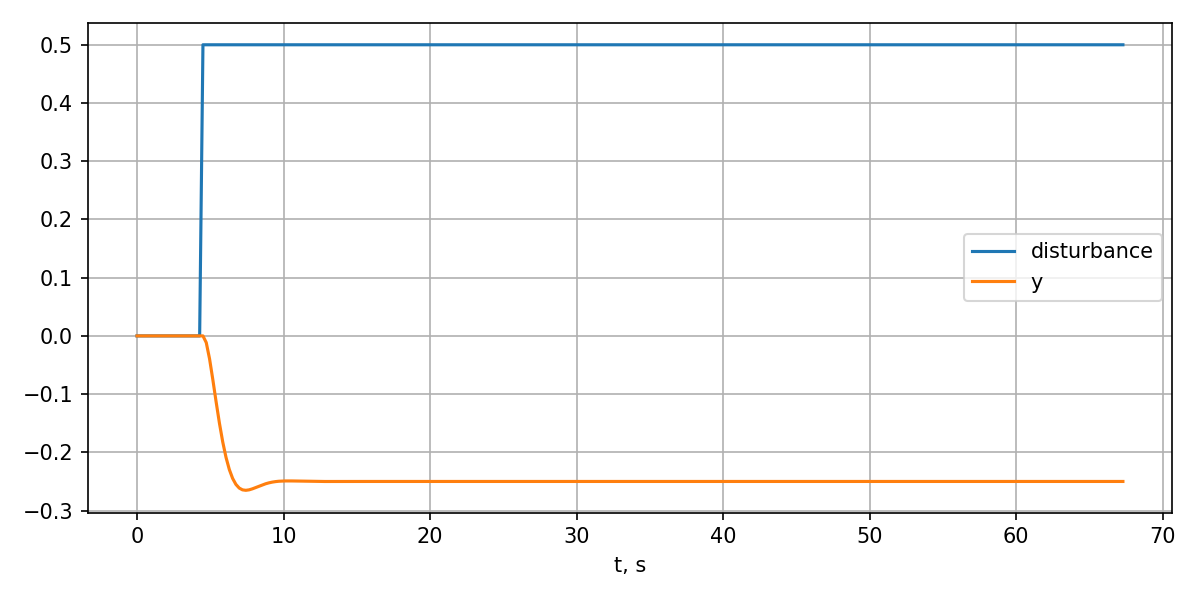
\includegraphics{task1/step_dist_T14.png}
    \caption{Ступенчатое возмущение, $T=T_1/4$}
\end{figure}

\begin{figure}[H]
    \centering
    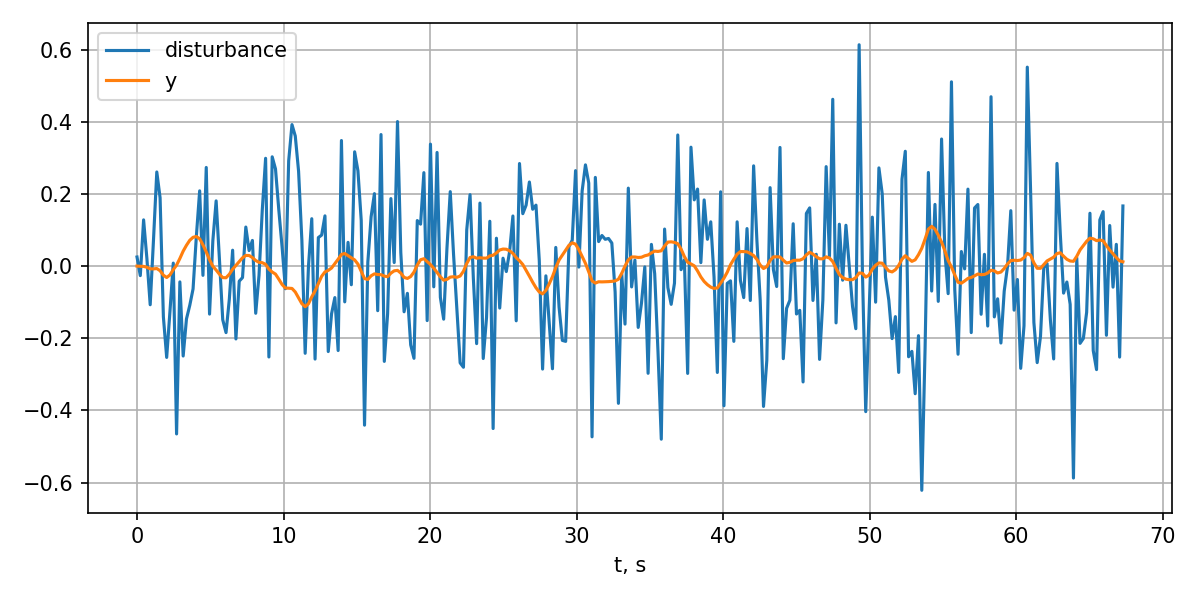
\includegraphics{task1/noise_T14.png}
    \caption{Случайное возмущение, $T=T_1/4$}
\end{figure}

\section{Влияние периода дискретизации и неточности $T_2$}
Сравниваются качества процесса управления при $T=T_1/2$ и $T=T_1/4$ (Рисунок ниже): уменьшение $T$ снижает дискретизационные искажения и ускоряет процесс, цена — более частое обновление управления. Также исследуется влияние неточности компенсации полюсов: $T_2$ изменяется на $\pm20\%$, реакции фиксируются при неизменном $q_0$ для режима $T=T_1/2$. При занижении/завышении $T_2$ наблюдаются соответственно более быстрые/замедленные переходные и изменение перерегулирования — это демонстрирует чувствительность САУ к ошибок идентификации.

\begin{figure}[H]
    \centering
    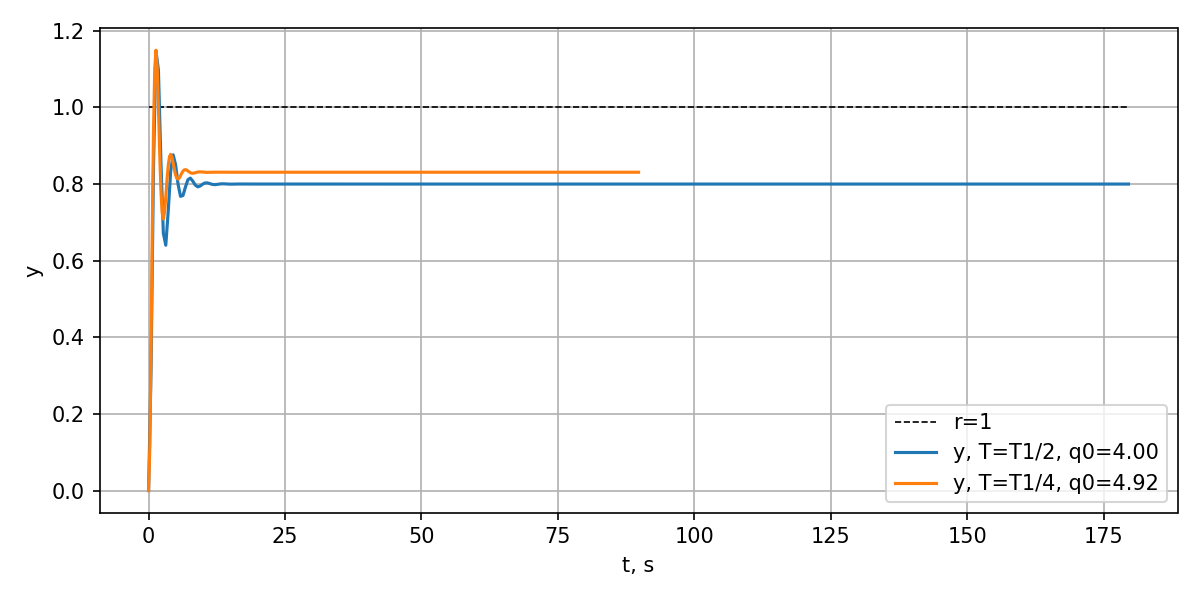
\includegraphics{task2/compare_T.png}
    \caption{Сравнение $T=T_1/2$ и $T=T_1/4$ (переходные по заданию)}
\end{figure}

\begin{figure}[H]
    \centering
    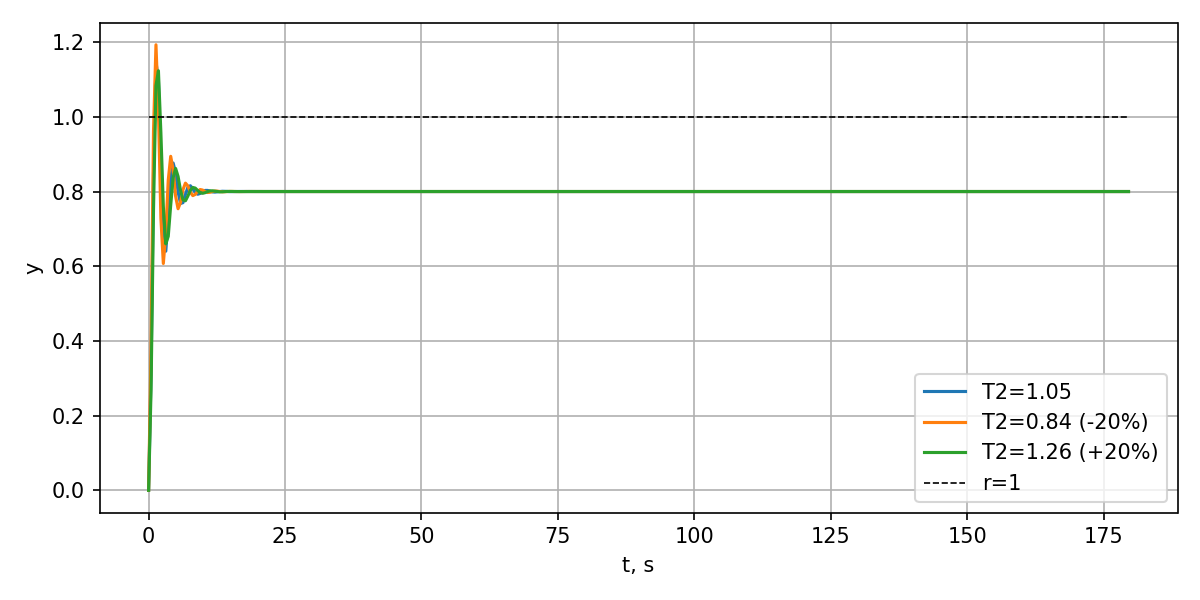
\includegraphics{task3/compare_T2_perturb.png}
    \caption{Влияние ошибки $T_2$ на реакцию на возмущение}
\end{figure}

\section{Выводы}
Получены следующие выводы: (i) $T=T_1/4$ обеспечивает лучшее качество (меньше ISE и время установления) при сопоставимом перерегулировании, чем $T=T_1/2$; (ii) корректный выбор $q_0$ позволяет добиться слабоколебательных переходных; (iii) ошибка в $T_2$ на $\pm20\%$ заметно влияет на быстродействие и перерегулирование, что требует уточнения модели в контуре настройки.


